\chapter{پیاده‌سازی سیستم}

در جهت اعمال نگهداری و تعمیرات پیش‌بینانه روی گره‌های موجود در اینترنت اشیاء، توسعه و پیاده‌سازی یک کارگزار برای دریافت درخواست‌ها و ارسال نتایج پیش‌بینی بسیار مفید است. با کمک این کارگزار همچنین فرایند‌های احراز هویّت\LTRfootnote{Authetication} و تایید\LTRfootnote{Verification} مدیران و دروازه‌ها نیز پیش‌برده خواهند شد. همچنین این کارگزار با بسته‌ی هوش مصنوعی که در فصل بعد به آن اشاره می‌کنیم، تعامل خواهد کرد.


\section{معماری مایکروسرویس}
یکی از معماری‌هایی که در سال‌های اخیر مورد توجه مهندسین نرم‌افزار قرار گرفته‌است، این معماری است که در آن هر کدام از بخش‌های سیستم در فضایی جدا شده و منزوی قرار می‌گیرند
و به صورت سرویس‌های کوچکی درمی‌آیند و هر کدام از این سرویس‌ها باهمدیگر در ارتباط می‌باشند. در این حالت  نیاز به یک سرویس اصلی مرکزی برای مدیریت سایر سرویس‌ها و ایجاد ارتباط میان آنها نیز می‌باشیم. از اصلی‌ترین نقاط مثبت این سیستم این است که می‌توان مشکل تضاد داشتن کتابخانه‌ها و نیازمندي‌های قسمت‌های مختلف را به سادگی رفع کرد. بدین صورت که هر سرویس دارای کتابخانه‌ها و نیازمنديی‌هایی که دارد می‌باشد و دیگر نیازی ندارد تا با بقیه‌ی سرویس‌ها تراز باشد. از مزایای دیگر این سیستم عیب‌یابی ساده‌تر آن به نسبت سیستم یکپارچه می‌باشد\cite{thones2015microservices}. در این پروژه سعی بر این بوده که تا حد ممکن، بخش‌های مختلف پروژه از هم جدا شوند تا بتوان از مزایای معماری مایکرو‌سرویس استفاده کنیم.

\subsection{داکر و داکرکامپوز}
اصلی‌ترین ابزار برای اعمال و پیاده‌سازی معماری مایکروسرویس، داکر می‌باشد. برای استفاده از آن پس از توسعه‌ی سرویس مورد نظر با کمک داکرفایل\LTRfootnote{Dockerfile}، ایمیج مربوط به سرویس را درست کرد و پس از آن بین سرویس‌های مختلف با کمک داکرکامپوز ارتباط برقرار کرد. داکرکامپوز به ما کمک می‌کند تا چندین کانتینر داکری را به راحتی مدیریت و اجرا کرد.

\subsection{سرویس کارگزار اصلی}
کارگزار اصلی به صورت بسته‌هایی شامل احراز هویّت، مدل یادگیری ماشین و تحلیل و آنالیز می‌باشد. پس از توسعه‌ی این سرور با کمک داکرفایل نمایش‌داده‌شده در \cref{fig:server_dockerfile}، ایمیج مربوط به این کارگزار را تولید کرده و از این پس به راحتی با کمک داکر و ایجاد کانتینر از این ایمیج، از آن استفاده می‌کنیم.

\begin{figure}[!h]
\centerline{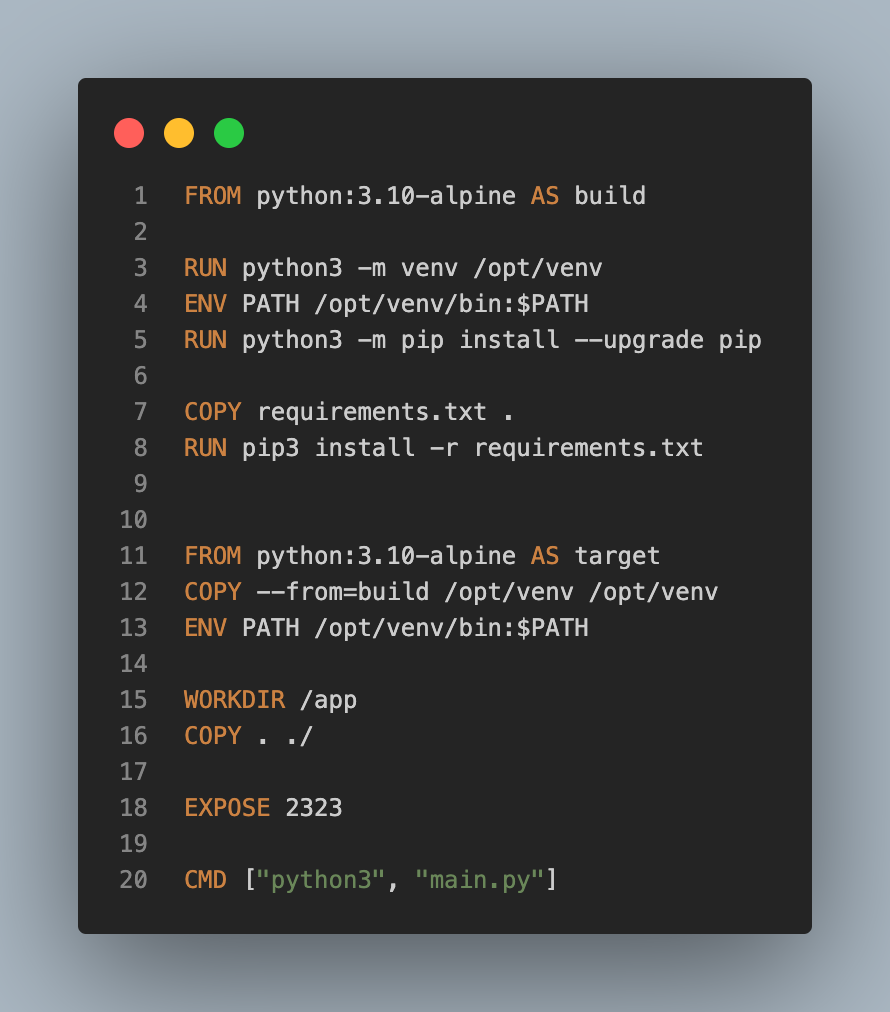
\includegraphics[width=0.6\textwidth]{server_dockerfile.png}}
\caption{داکرفایل مربوط به کارگزار اصلی}
\label{fig:server_dockerfile}
\end{figure}

\subsection{سرویس‌های پایگاه داده}
پس از پیاده‌سازی کارگزار اصلی، هرکدام از پایگاه‌ داده‌های رابطه‌ای و غیر رابطه‌ای را به عنوان یکی سرویس اضافه و مستقل از کارگزار، توسط داکرکامپوز نشان‌داده‌‌شده در \cref{fig:docker_compose} توسعه دادیم و به کارگزار اصلی در یک شبکه‌ی داخلی متصل کردیم.

\begin{figure}[!h]
\centerline{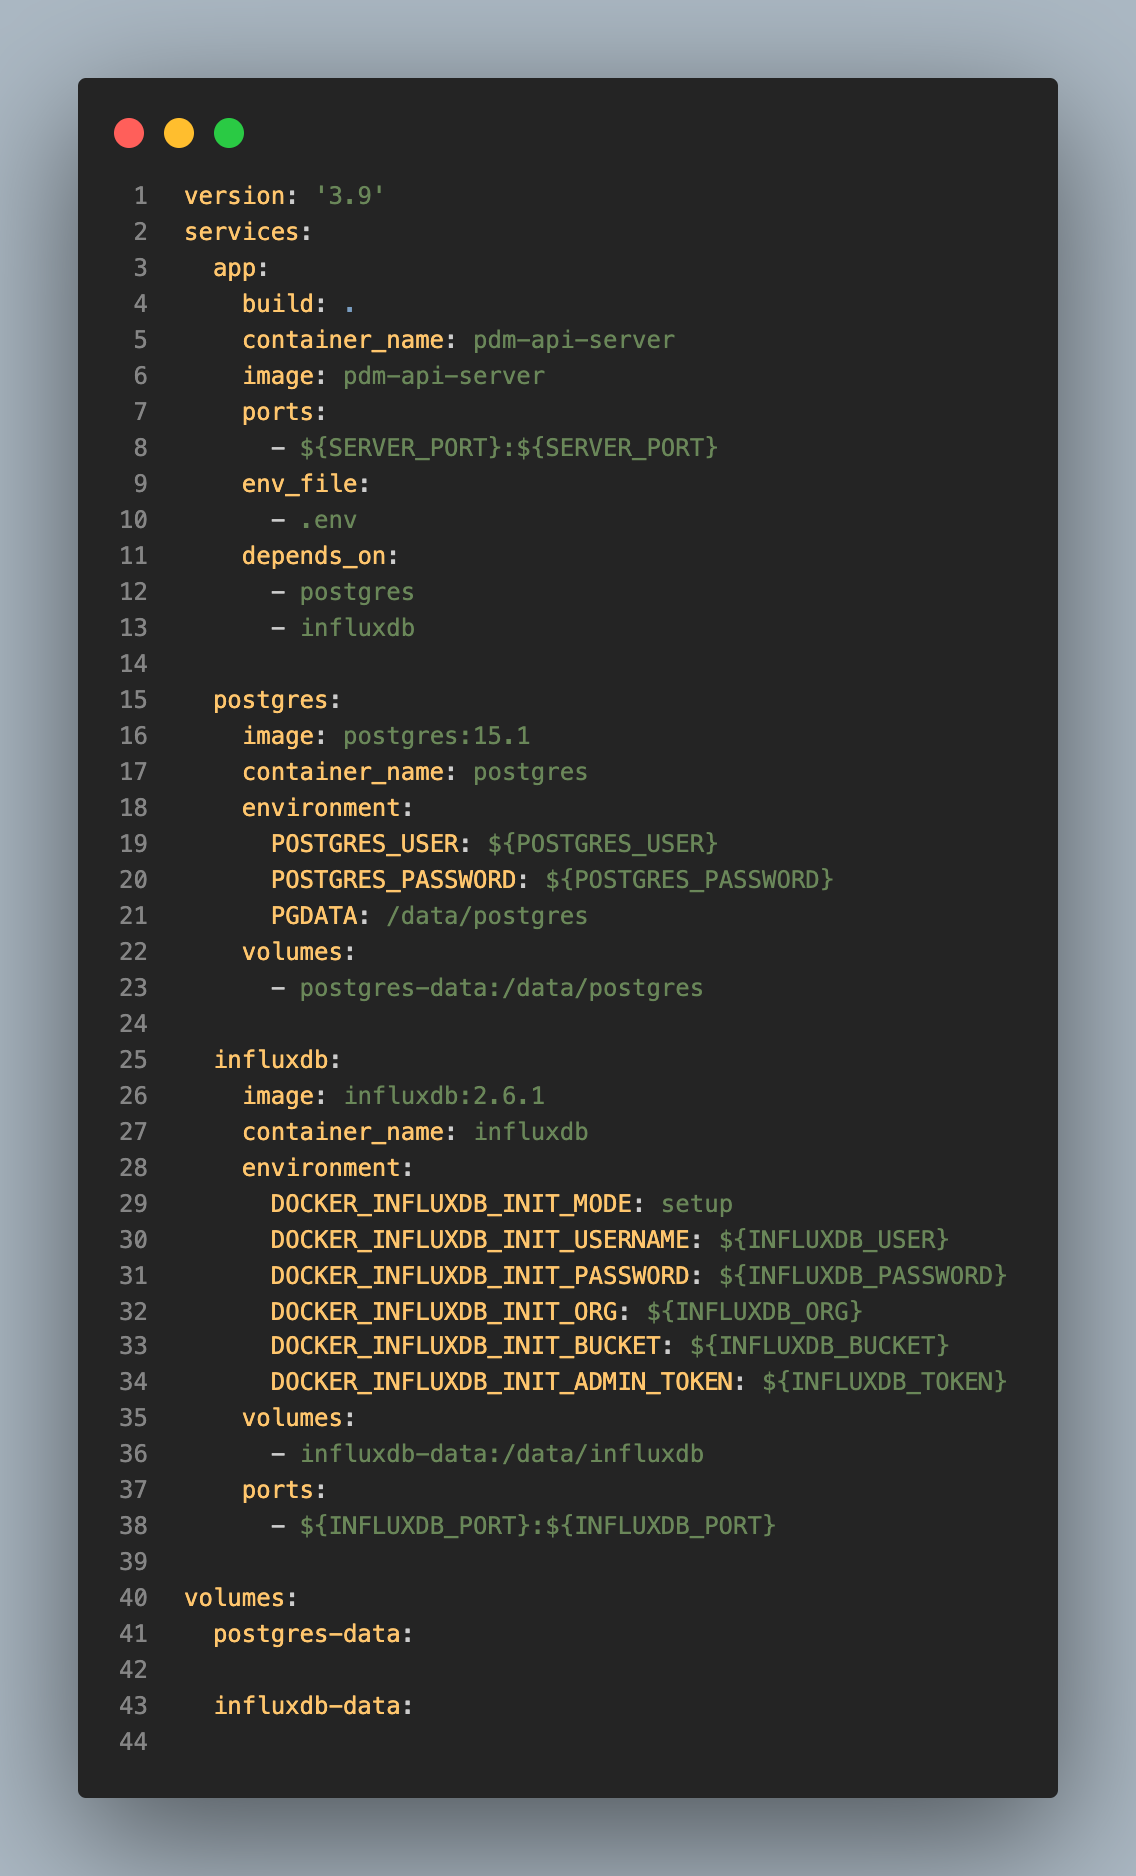
\includegraphics[width=0.6\textwidth]{docker_compose.png}}
\caption{داکرکامپوز مربوط به سیستم نهایی}
\label{fig:docker_compose}
\end{figure}


\section{معماری سیستم}
در این قسمت ابتدا بخش‌های مختلف سیستم را نشان می‌دهیم سپس به توضیح هر کدام از قسمت‌ها خواهیم پرداخت. همانطور که در \cref{fig:system_architecture} می‌بینیم، سیستم نگهداری پیش‌بینانه طراحی‌شده به طور کلی از چهار بخش تقسیم‌شده است. کارگزار اصلی که رابط بین مدیران و دروازه‌ها با مدل یادگیری ماشین است و وظیفه‌ دارد به طور مشخص و دقیق درخواست مربوط به هر کدام از کاربران را پاسخ دهد. مهم‌ترین قسمت این سیستم، بسته‌ی هوش مصنوعی می‌باشد که با کارگزار اصلی و پایگاه‌ داده‌ی سری زمانی در ارتباط است و نتایج تحلیل‌ها و پیش‌بینی‌ها را به این دو ابلاغ می‌کند. نکته‌ی شایان توجه در این قسمت این است که به ازای هر باز آموزش جدید مدل، داده‌ها به مدت ۱۵ دقیقه در پایگاه‌ داده‌ی سری زمانی ذخیره می‌شوند تا سرعت پاسخ‌دهی به کاربران برای درخواست‌های تکراری افزایش یابد.

\begin{figure}[!h]
\centerline{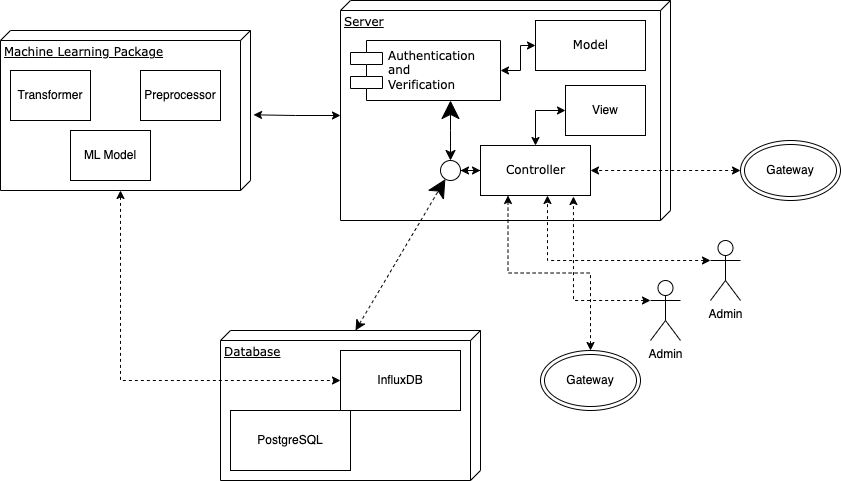
\includegraphics[width=\textwidth]{system_architecture.png}}
\caption{معماری کلی سیستم طراحی‌شده}
\label{fig:system_architecture}
\end{figure}


در \cref{fig:system_structure} انواع بسته‌های پایتونی مجزا از هم توسعه‌داده‌شده برای سیستم نگهداری پیش‌بینانه را مشاهده می کنیم. در این قسمت، هر کدام از این بخش‌ها را تشریح می‌کنیم.

\subsection{بسته‌ی \lr{auth}}
وظیفه‌ی این بخش انجام همه‌ی کارهای احراز هویّت و تایید کاربران است. همچنین توابع تولید هش رمز عبور کاربران جدید نیز در این بخش پیاد‌ه‌شده است.

\subsection{بسته‌ی \lr{influxdb}}
همه‌ی فایل‌ها و کلاس‌های لازم برای ارتباط با و استفاده از پایگاه‌داده‌ی سری زمانی، در این بسته قرار دارند. تمام کارهای خواندن و نوشتن داده‌ها و نتایج مدل یادگیری ماشین در این بخش مدیریت می‌شوند. این بخش از آنجا که هم با کارگزار اصلی و هم با بسته‌ی یادگیری ماشین در تعامل است، گلوگاه سیستم حساب می‌شود و ممکن است درخواست‌های زیاد را به خوبی نتواند مدیریت کند. از این رو در طی پیاده‌سازی این پروژه سعی بر این بوده که این بخش کارایی و سرعت لازم را داشته‌ باشد و در نوشتن پرس‌وجوهای پایگاه داده در این بخش، نهایت دقت به عمل آمده است.

\subsection{بسته‌ی \lr{models}}
این بسته شامل شمای کلی شی‌ء‌های در‌خواست‌های کاربران و پاسخ‌های منتسب به آنها است\cite{deacon2009model}. تمامی درخواست‌هایی که به سمت کارگزار اصلی ارسال می‌شوند باید اشیائی طبق شمای بیان‌شده در این بخش را داشته‌ باشند. همچنین ساختار پاسخ‌های کارگزار به کاربران در این قسمت قرار داده‌شده است.

\subsection{بسته‌ی \lr{postgresdb}}
این بسته نیز شامل همه‌ی فایل‌های لازم برای ایجاد ارتباط با پایگاه‌ داده‌ی رابطه‌ای است. در قسمت‌های بعد بیشتر با این بسته آشنا خواهیم شد.

\subsection{بسته‌ی \lr{routers}}
همه‌ی نقاط انتهایی‌ای که در دسترس کاربران قرار گرفته‌اند، در این بخش پیاده و توصیف شده‌اند. همانطور که در \cref{fig:system_structure} می‌بینیم، برای هر کدام از کارهای ورود، ثبت‌نام، تایید، آنالیز و تحلیل و همچنین ارسال و دریافت داده نقاط نهایی مشخصی تعبیه ‌شده‌اند. در \cref{fig:endpoints} تعدادی از این نقاط انتهایی را برای تایید مدیران و دروازه‌ها، دریافت و ارسال داده‌های لرزش و ورود کاربران، مشاهده می‌کنیم. نکته‌ی قابل‌توجه در این بخش این است که الگوی پیاده‌شده در این قسمت، بر اساس الگوی مدل-نما-کنترل‌گر\cite{deacon2009model} می‌باشد و این بسته شامل دو بخش نما و کنترل‌گر است.

\subsection{بسته‌ی \lr{utils}}
این بسته نیز شامل مواردی است که در کل سامانه مورد استفاده قرار می‌گیرند. این موارد شامل متغیر‌های محیطی\LTRfootnote{Environment Variables}، متغیر‌های ثابت و پارامتر‌های ثابت مدل یادگیری ماشین هستند.

\begin{figure}[!h]
\centerline{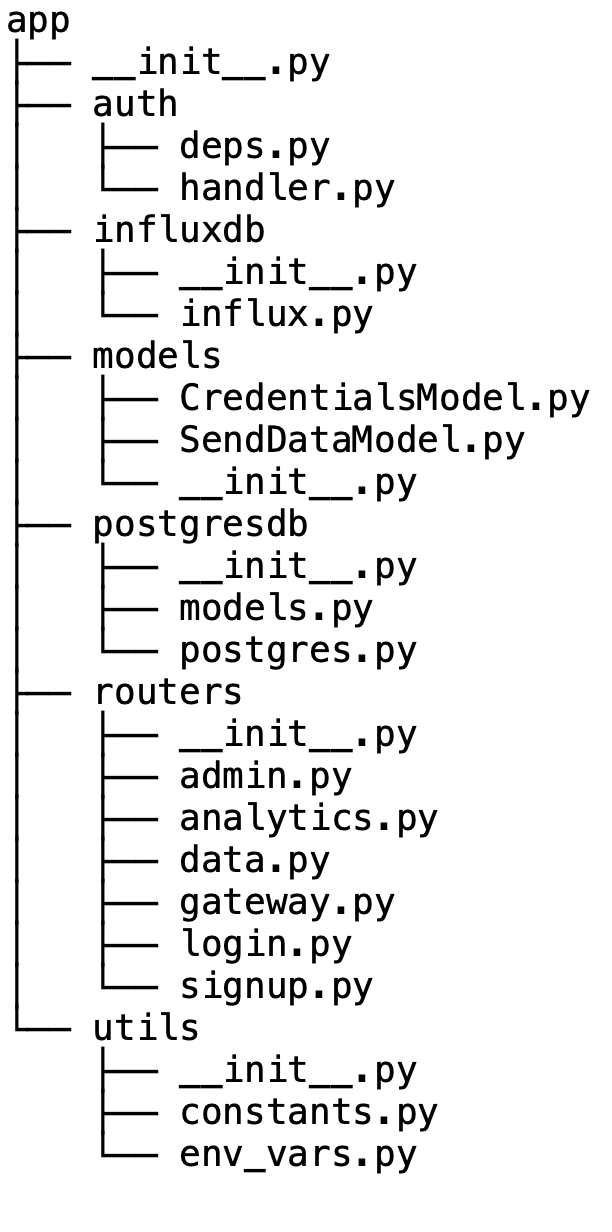
\includegraphics[width=0.5\textwidth]{system_structure.png}}
\caption{ساختار بسته‌های سیستم}
\label{fig:system_structure}
\end{figure}

\begin{figure}[!h]
\centerline{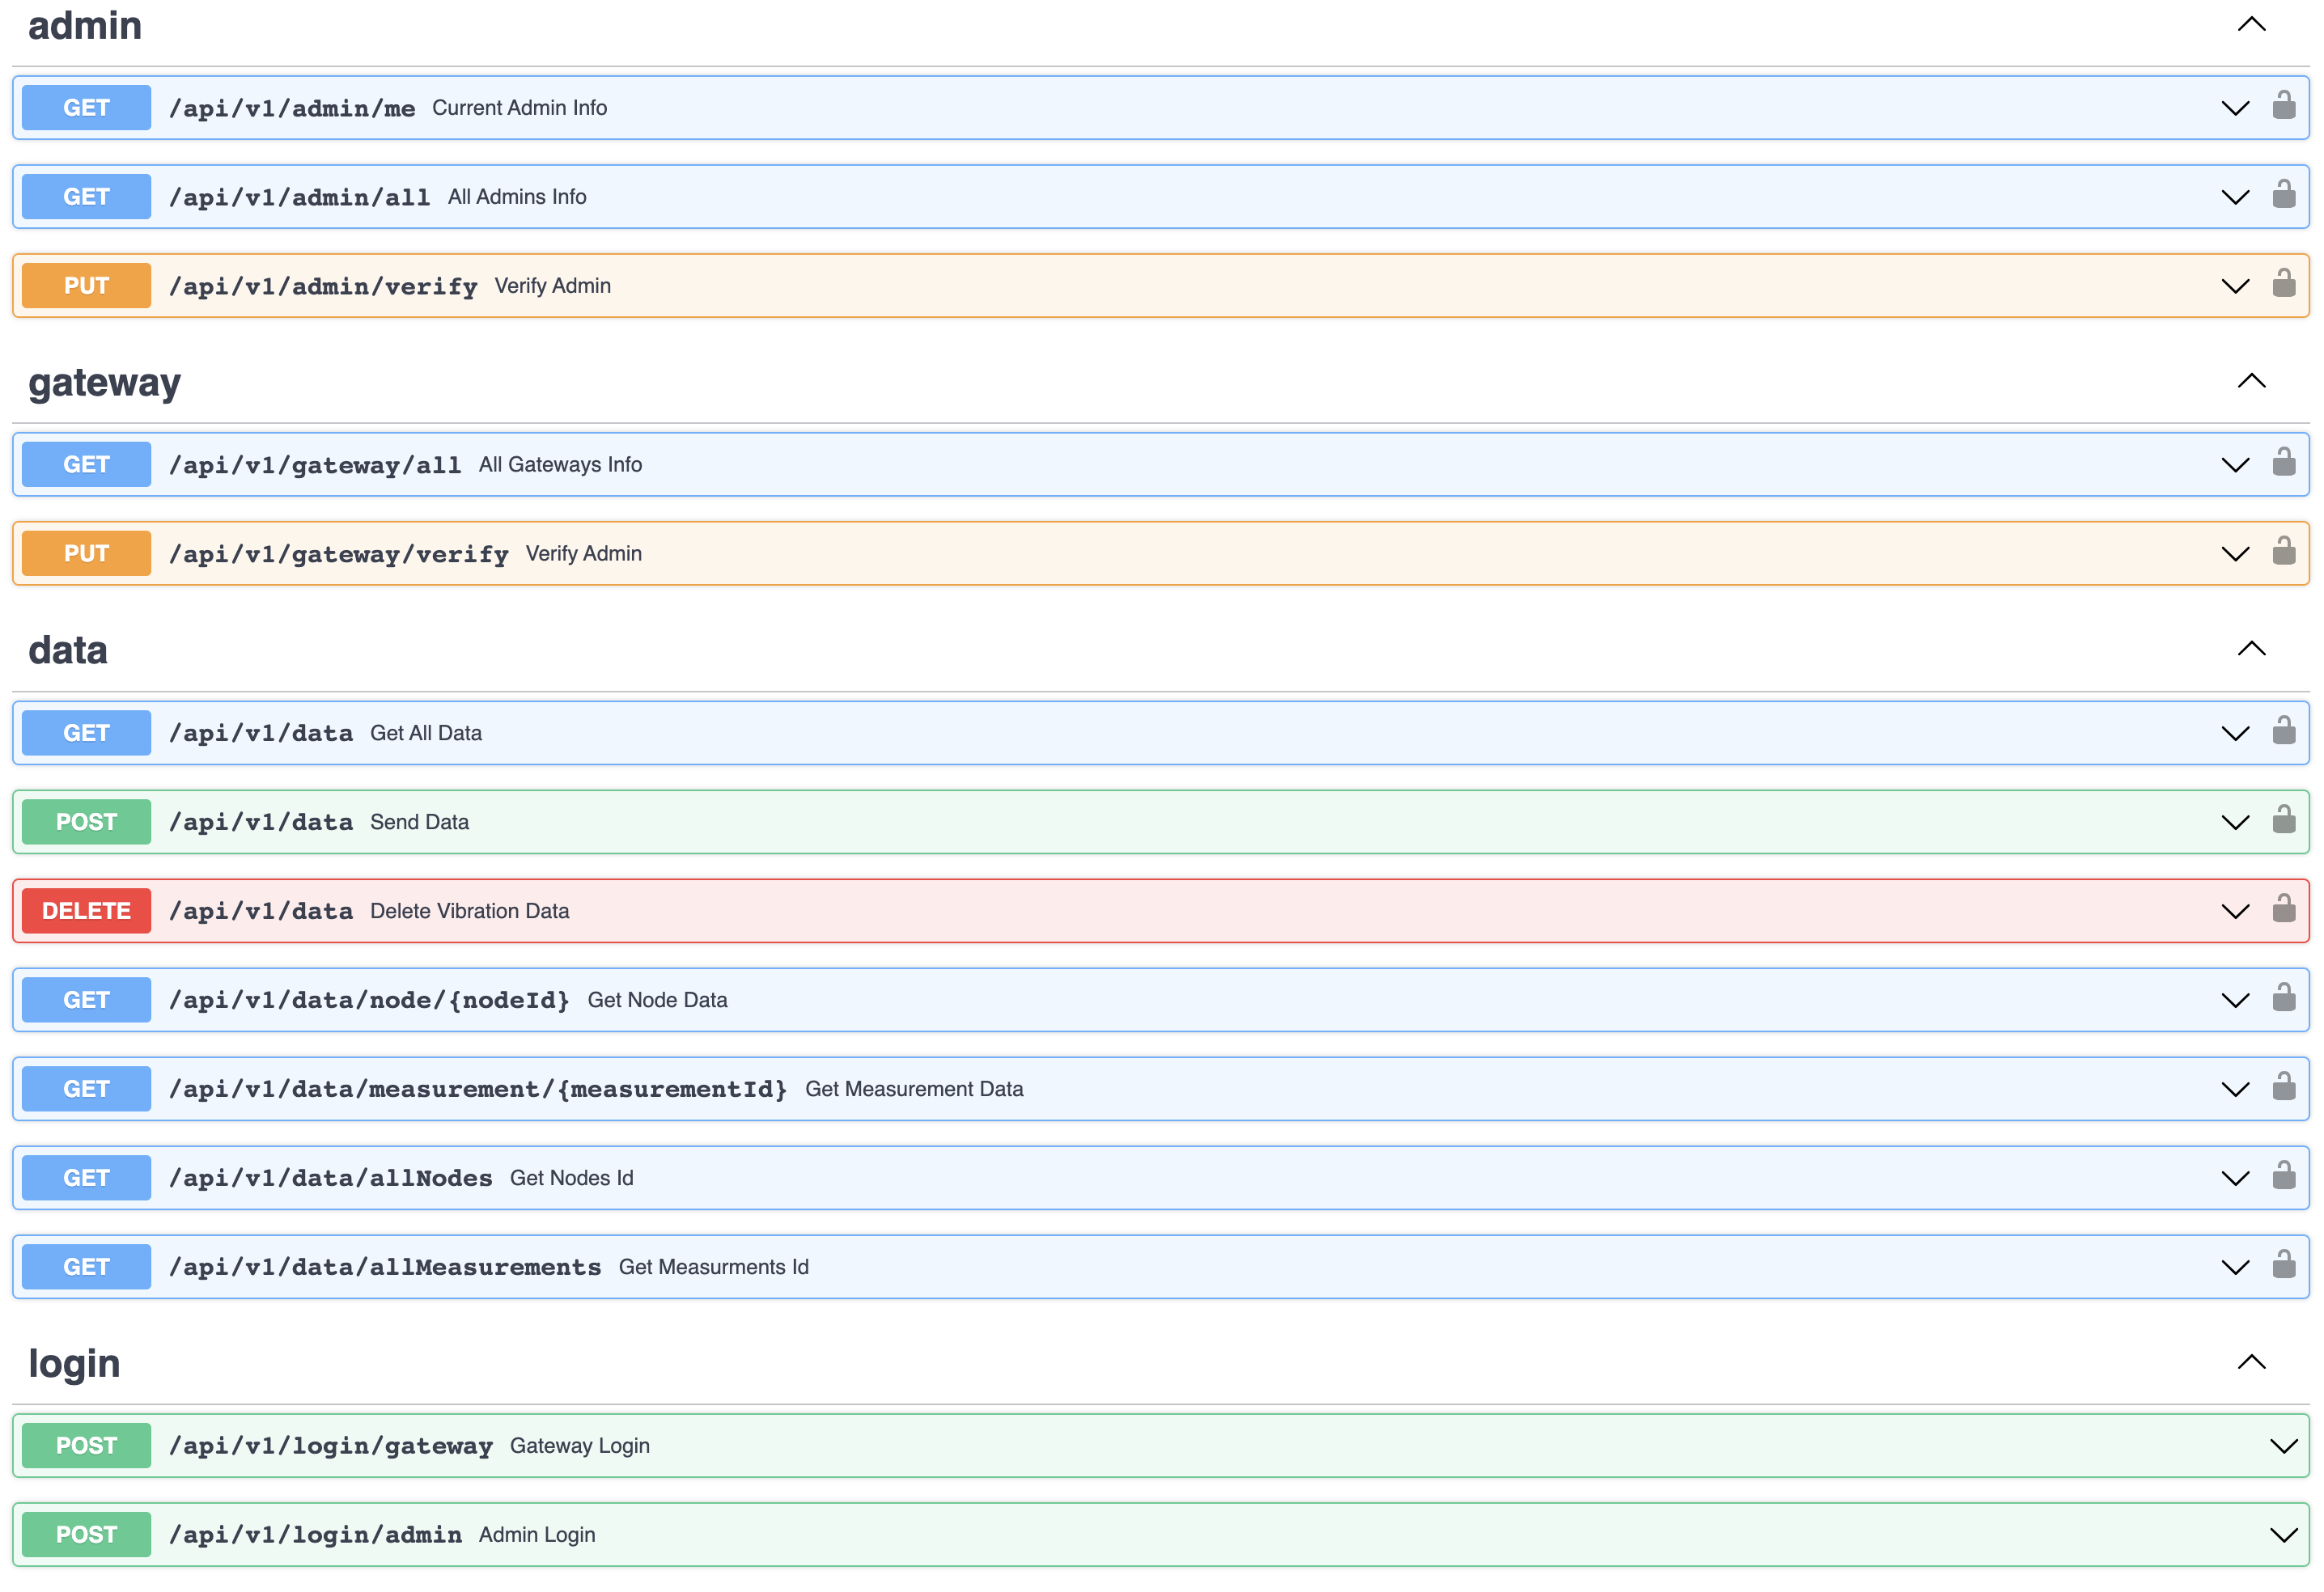
\includegraphics[width=\textwidth]{endpoints.png}}
\caption{تعدادی از نقاط انتهایی سامانه}
\label{fig:endpoints}
\end{figure}


\section{پایگاه داده‌ی رابطه‌ای}
برای مدیریت و نگهداری اطلاعات مدیران و دروازه‌ها در این پروژه از پایگاه داده‌ی رابطه‌ای متن‌باز \lr{PostgreSQL} استفاده کرده‌ایم. تنها، بخش نما از کارگزار اصلی به این پایگاه داده دسترسی دارد و عملیات احراز هویت و همچنین مدیریت دسترسی کاربران برای دیدن یا درخواست انجام پیش‌بینی‌ها و تحلیل‌ها و صدور مجوز برای ارسال داده‌های حسگرهای لرزش از سمت دروازه‌ها به کارگزار اصلی با کمک این بخش انجام خواهد شد. در \cref{table:admins} و \cref{table:gateways} به ترتیب شمای مربوط به جداول مدیران و دروازه‌ها را مشاهده می‌کنیم.

\begin{table}[h!]
  \begin{center}
    \caption{شمای جدول مدیران}
    \label{table:admins}
    \begin{tabular}{|c|c|} % <-- Alignments: 1st column left and 2nd right with vertical lines in between
    	\hline
\multicolumn{2}{|c|}{\textbf{مدیر}}\\ \hline\hline
\textbf{توضیحات} & \textbf{ستون}\\
    	\hline
	عددی یکتا برای هر مدیر & شناسه\\
    	\hline
	رشته‌ای یکتا برای هر مدیر & ایمیل\\
    	\hline
رشته‌ای هش‌شده برای ورود هر مدیر به سیستم & رمز عبور\\
    	\hline
به صورت رشته & نام\\
    	\hline
متغیری صفر و یکی & تایید‌شده\\
    	\hline
زمان ثبت‌نام مدیر & ثبت‌نام در\\
    	\hline
زمان آخرین ورود مدیر به سیستم & آخرین ورود در\\
    	\hline
زمان تایید مدیر توسط یک مدیر تایید‌شده & تایید شده در\\
    	\hline
    \end{tabular}
  \end{center}
\end{table} 

\begin{table}[h!]
  \begin{center}
    \caption{شمای جدول دروازه‌ها}
    \label{table:gateways}
    \begin{tabular}{|c|c|} % <-- Alignments: 1st column left and 2nd right with vertical lines in between
    	\hline
\multicolumn{2}{|c|}{\textbf{دروازه}}\\ \hline\hline
\textbf{توضیحات} & \textbf{ستون}\\
    	\hline
	عددی یکتا برای هر دروازه & شناسه\\
    	\hline
آدرسی فیزیکی یکتای منسوب به هر دروازه & آدرس فیزیکی\\
    	\hline
رشته‌ای هش‌شده برای ورود هر دروازه به سیستم & رمز عبور\\
    	\hline
متغیری صفر و یکی & تایید‌شده\\
    	\hline
زمان ثبت‌نام دروازه & ثبت‌نام در\\
    	\hline
زمان آخرین ورود دروازه به سیستم & آخرین ورود در\\
    	\hline
زمان تایید دروازه توسط یک مدیر تایید‌شده & تایید شده در\\
    	\hline
    \end{tabular}
  \end{center}
\end{table} 

\section{امنیت}
یکی از مهم‌ترین ویژگی‌های سیستم طراحی‌شده که وجه تمایز بین این پروژه را با دیگر پروژه‌های مشابه ایجاد می‌کند، پیاده‌شدن لایه‌ها مختلف امنیت در این پروژه است. همه‌ی مدیران و دروازه‌ها پس از ثبت‌نام و ایجاد حساب کاربری باید توسط مدیران تایید‌شده تایید شوند تا دسترسی‌های خود را پیدا کنند. همچنین برای احراز هویّت هر کدام از مدیران و دروازه‌ها تدابیری اندیشیده‌ایم که در قسمت‌های زیر به آنها اشاره خواهیم کرد.

\subsection{احراز هویّت}
برای شناسایی و احراز هویّت کاربران این سیستم از استاندارد \lr{JWT}\LTRfootnote{JSON Web Token} بهره برده‌ایم. از این استاندارد برای ایجاد داده‌ی رمزشده با یک امضا\LTRfootnote{Signature}ی مشخص استفاده می‌شود. این نشانه‌ها یا توسط یک رمز خصوصی یا با کلید عمومی خصوصی امضا می‌شوند. هر نشانه‌ شامل سه بخش سرآمد\LTRfootnote{Header}، بدنه‌ی اصلی\LTRfootnote{Payload} و امضا می‌باشد\cite{jones2015json}. نکته‌ی قابل‌ توجه این است که هر گونه تغییر در بدنه‌ی اصلی نشانه، امضای نشانه را بهم می‌زند و پیام ارزش قانونی خود را از دست خواهد داد. در واقع کارگزار اصلی پس از هر بار دریافت نشانه‌ از سمت کاربران، بررسی می‌کند که آیا خود این پیام را امضا کرده است یا خیر. اگر این پیام توسط خودش امضا نشده‌ باشد، درخواست کاربر را بررسی نخواهد کرد.

\subsubsection{سرآمد}
در سرآمد نشانه، اطلاعات مربوط به الگوریتم استفاده‌شده برای ایجاد امضا آورده می‌شود. در قسمت زیر نمونه‌ای از سرآمد یک نشانه‌ی \lr{JWT} را مشاهده می‌کنیم. همانطور که مشخص است، از الگوریتم \lr{HMAC-SHA256} برای امضای بدنه‌ی اصلی این پیام استفاده‌شده است.

\begin{latin}
\begin{lstlisting}[language=json,firstnumber=1]
{
  "alg": "HS256",
  "typ": "JWT"
}
\end{lstlisting}
\end{latin}

\subsubsection{بدنه‌ی اصلی}
این قسمت شامل تعدادی از ادعاهاست که فرد دارنده‌ی نشانه می‌تواند از آن استفاده کند. در قسمت زیر نمونه‌ای از یک نشانه‌ی صادر شده برای یکی از مدیران و زمان انقضای این نشانه را مشاهده می‌کنیم. نکته‌ی قابل توجه این است که پس از زمان نشان‌داده‌شده، نشانه دیگر کارایی ندارد و درخواست‌هایی که شامل این نشانه هستند، بررسی نخواهند شد.

\begin{latin}
\begin{lstlisting}[language=json,firstnumber=1]
{
  "email": "user@example.com",
  "exp": 1689956613
}
\end{lstlisting}
\end{latin}

\subsubsection{امضا}
این قسمت به صورت امن، قانونی‌بودن نشانه‌ی صادر شده را تضمین می‌کند. این امضا، توسط رمزشدن رشته‌ی تغییر‌یافته توسط \lr{Base64} سرآمد و بدنه‌ی اصلی با کمک الگوریتم مشخص‌شده در سرآمد و با یک رمز خصوصی در سمت کارگزار تولید می‌شود. هنگامی که کارگزار نشانه‌ای را دریافت می‌کند، ابتدا امضای آن را با امضای صادرشده برای آن مقایسه می‌کند و در صورت یکی بودن آنها درخواست بررسی خواهد شد.


\subsection{تایید مدیران و دروازه‌ها}
هر یک از مدیران و دروازه‌های تازه ثبت‌نام کرده باید توسط یکی از مدیران تایید‌ و احراز هویت‌شده، تایید شوند. پس از تایید، مدیران می‌توانند به نتایج تحلیل‌ها و داده‌های بدست‌آمده توسط مدل یادگیری ماشین دسترسی پیدا کنند. از طرفی دروازه‌ها نیز پس از این عمل، توانایی ارسال داده‌های جمع‌آوری‌شده توسط خود را پیدا خواهند کرد. 

\section{جمع‌بندی و نتیجه‌گیری}
در این بخش از نوشته، با معماری کلی سامانه‌ی طراحی‌شده برای اعمال نگهداری پیش‌بینانه روی گره‌های اینترنت اشیاء آشنا شدیم. همانطور که دیدیم، این سیستم طبق معماری مایکروسرویس، شامل چندین بخش مجزا پیاده‌شده است. همچنین دیدیم که الگوی بکار‌رفته برای طراحی کارگزار الگوی مدل-نما-کنترل‌گر بود و نتایج درخواست‌ها طبق این الگو تحویل کاربران داده می‌شوند. در مرحله‌ی آخر نیز دو سرویس پایگاه داده‌ی رابطه‌ای و امنیت را تشریح کردیم. در فصل بعد، مهم‌ترین مؤلفه‌ی سیستم کنونی، یعنی سرویس یادگیری ماشین را تجزیه و تحلیل خواهیم کرد.